\section{Generalized Linear Models}
\subsection{Overview and Data}
\begin{frame}\frametitle{Beyond Linear Models}
  \begin{itemize}
  \item linear models are central to the practice of statistics
  \item the standard linear model cannot handle non-normal responses, such as counts or proportions. This motivates the development of
\textit{generalized linear models} that can represent categorical, binary and other response types.
  \end{itemize}
\end{frame}

\begin{frame}\frametitle{Beyond Linear Models}
  \begin{itemize}
  \item Some data has a grouped, nested or hierarchical structure. Repeated measures, longitudinal and multilevel data consist of several observations taken
on the same individual or group. This induces a correlation structure in the error. \textit{mixed effect models} allow the modeling of such data.
  \item \textit{non-parametric regression models}: Methods such as additive models, trees and neural networks allow a more flexible regression
modeling of the response that combine the predictors in a nonparametric manner.
  \end{itemize}
\end{frame}

\begin{frame}[fragile]\frametitle{Generalized Linear Models}
Linear modeling assumes constant variance and normally distributed errors. Certain kinds of respond variables lack these constraints. GLMs are excellent at dealing with it.
\begin{exampleblock}{Input/Output}\small
\begin{verbatim}
> m1 <- lm(bweight ~ hyp, data=births)
> m2 <- glm(bweight ~ hyp, family=gaussian, data=births)
\end{verbatim}
\end{exampleblock}
give the same answer. The model formula is the same for both, but for \texttt{glm()} it is necessary to specify the family of likelihoods which will be used to fit the model. 

The \texttt{glm()} function allows us to fit other models including logistic regression and Poisson regression.
\end{frame}

\begin{frame}\frametitle{Beyond Linear Models}
  \begin{itemize}
    \item We begin with a binary response variable:
  \end{itemize}
\end{frame}

\subsection{Binary Response Variables}

\begin{frame}\frametitle{Bernoulli model}
  \begin{itemize}
  \item $f(y;p) = p^y(1-p)^{1-y}$
  \item it is modelled with a logit as canonical link $$ \eta = \log(\frac{p}{1-p})$$
  \item i.e. our linear model looks like $$ \eta = \log(\frac{p}{1-p}) = \beta_0 + \beta_1 x_1 + \cdots + \beta_n x_n + \epsilon$$ with a binomial error structure
  \end{itemize}
\end{frame}



\begin{frame}[fragile]\frametitle{Data Structure}
Load the data ~birthsweights.rdata~. 
The structure of the data should be of the following form:
\footnotesize
\begin{exampleblock}{Input/Output}
\begin{semiverbatim}
    > str(births)
    'data.frame':	500 obs. of  8 variables:
    $ id     : num  100 101 102 103 104 105 106 107 108 109 ...
    $ preterm: chr  "normal" "normal" "normal" "normal" ...
    $ gestwks: num  39.8 39 38.1 39.5 39.5 ...
    $ hyp    : chr  "normal" "normal" "normal" "normal" ...
    $ matage : num  33 32 33 38 40 29 32 40 41 39 ...
    $ bweight: num  3576 3784 2796 3226 3138 ...
    $ lowbw  : chr  "normal" "normal" "normal" "normal" ...
    $ sex    : chr  "F" "F" "F" "F" ...
\end{semiverbatim}
\end{exampleblock}
Data from: Michael Hills and Bianca De Stavola (2002). A Short Introduction
     to Stata 8 for Biostatistics, Timberlake Consultants Ltd URL:
     http://www.timberlake.co.uk
\end{frame}


\begin{frame}\frametitle{Binary Response Variable}
Many statistical problems involve binary response variables. For example, we often classify individuals as:
\begin{itemize}
\item dead or alive,
\item occupied or empty,
\item healthy or diseased,
\item wilted or turgid,
\item male or female,
\item literate or illiterate,
\item mature or immature,
\item solvent or insolvent, or
\item employed or unemployed.
\end{itemize}
\end{frame}

\begin{frame}\frametitle{Binary Response Variable}
\begin{block}{Question}
Which variable in the births data set is (most) suitable to use as binary response given this data set? Why?
\end{block}
\end{frame}


\begin{frame}[fragile]\frametitle{Predicting Low Birth Weight}
\begin{itemize}
\item Now we are more interested in predicting birth weight under 2500g (\texttt{lowbw}). 
\item This requires a model where the outcome is not metric, but binary. 
\item For a binary response we use a \texttt{glm()} with a \emph{binomial} family.
\item the \emph{binomial} family uses  a \emph{logit} link as default
\end{itemize}
\end{frame}


\begin{frame}[fragile]\frametitle{Predicting Low Birth Weight}\footnotesize
How it looks in R:
\begin{exampleblock}{Input/Output}\scriptsize
\begin{verbatim}
> m <- glm(lowbw ~ hyp, family=binomial, data=births)
> summary(m)
Call:
glm(formula = lowbw ~ hyp, family = binomial, data = births)

Deviance Residuals: 
    Min       1Q   Median       3Q      Max  
-0.8067  -0.4430  -0.4430  -0.4430   2.1773  

Coefficients:
            Estimate Std. Error z value Pr(>|z|)    
(Intercept)  -2.2721     0.1661 -13.682  < 2e-16 ***
hyphyper      1.3166     0.3111   4.232 2.32e-05 ***
---

(Dispersion parameter for binomial family taken to be 1)

    Null deviance: 366.92  on 499  degrees of freedom
Residual deviance: 350.84  on 498  degrees of freedom
AIC: 354.84

\end{verbatim}
\end{exampleblock}
\end{frame}


\begin{frame}[fragile]\frametitle{Predicting Low Birth Weight}\footnotesize
What it looks like as a math formula:
$$ \log\left(\frac{\mbox{Pr(lowbw)}}{1-\mbox{Pr(lowbw)}}\right) = \beta_0 + \beta_1 \cdot \mbox{hyp} + \epsilon$$
\end{frame}


\begin{frame}[fragile]\frametitle{Interpreting the Coefficients}
\begin{itemize}
\item While using a binomial family R uses a logit as link function.
\item Therefore the returned estimates are log odds (Intercept) or log odds ratios (for the parameters). 
\item The \texttt{arm} package contains a function \texttt{invlogit()} which does invert the logit function. 
\item Alternatively you can use the formula $$ \mbox{logit}^{-1}= \frac{\exp(x)}{1+\exp{x}} $$
\end{itemize}
\end{frame}




\begin{frame}[fragile]\frametitle{Interpreting the Coefficients}
\begin{itemize}
\item Our example is a simple analysis of variance. 
\item Our model here is $$\mbox{Pr(lowbw)}=\mbox{logit}^{-1}(-2.2721 + 1.3166 \cdot \mbox{hyp})$$
\item We have two levels of our predictor variable \texttt{hyp}: \emph{normal} and \emph{hyp}. 
\item For the reference level \emph{normal} $\mbox{hyp}=0$ 
\item in this case we get \small $$\mbox{Pr(lowbw)}=\mbox{logit}^{-1}(-2.2721 + 1.3166 \cdot 0) = \mbox{logit}^{-1}(-2.2721)$$ which is a log odds as mentioned before, so 
  \begin{exampleblock}{Input/Output}
\begin{verbatim}
> invlogit(coef(m)[1]) 
(Intercept) 
 0.09345794 
\end{verbatim}
  \end{exampleblock}
\end{itemize}
\end{frame}

\begin{frame}[fragile]\frametitle{Interpreting the Coefficients}
\begin{itemize}
\item The result is the probability of low birth weight within the group of moms with normal blood pressure. We can check this by using \texttt{table}:
  \begin{exampleblock}{Input/Output}
\begin{verbatim}
> table(births$lowbw,births$hyp)
        
         normal hyper
  normal    388    52
  low        40    20
> 40/(388+40)
[1] 0.09345794
\end{verbatim}
  \end{exampleblock}
\end{itemize}
\end{frame}

\begin{frame}[fragile]\frametitle{Interpreting the Coefficients}
\begin{itemize}
\item for the level \emph{hyp} (i.e. $\mbox{hyp}=1$) we get a difference of $1.3166$ on the logit scale $$\mbox{Pr(lowbw)}=\mbox{logit}^{-1}(-2.2721 + 1.3166 \cdot 1) $$
\item which turns out to be
  \begin{exampleblock}{Input/Output}
\begin{verbatim}
> invlogit(coef(m)[1]+coef(m)[2])
(Intercept) 
  0.2777778 
\end{verbatim}
  \end{exampleblock}
\item so the probability for low birth weight is 27.8\% in for moms with high blood pressure
\end{itemize}
\end{frame}

\begin{frame}[fragile]\frametitle{Understanding the Coefficients}
\begin{itemize}
\item in this simple case, the response variable gives the probability for low birth weight for each of the two groups of moms (with and without high blood pressure)
\item you can get the result also using (a) a proportion test:\small
  \begin{exampleblock}\scriptsize
\begin{verbatim}
> prop.test(c(20,40),c(72,428))

	2-sample test for equality of proportions with continuity correction

data:  c(20, 40) out of c(72, 428)
X-squared = 18.121, df = 1, p-value = 2.073e-05
alternative hypothesis: two.sided
95 percent confidence interval:
 0.06913673 0.29950294
sample estimates:
    prop 1     prop 2 
0.27777778 0.09345794 
\end{verbatim}
  \end{exampleblock}
\end{itemize}
\end{frame}

\begin{frame}[fragile]\frametitle{Understanding the Coefficients}
\begin{itemize}
\item or (b) a $\chi^2$-test:\small
  \begin{exampleblock}{Input/Output}\footnotesize
\begin{verbatim}
> chisq.test(table(births$lowbw,births$hyp))

	Pearson's Chi-squared test with Yates' continuity correction

data:  table(births$lowbw, births$hyp)
X-squared = 18.121, df = 1, p-value = 2.073e-05
\end{verbatim}
  \end{exampleblock}
\end{itemize}
\end{frame}

\begin{frame}[fragile]\frametitle{Understanding the Coefficients}
\begin{itemize}
\item a \emph{hand made} plot
\begin{center}
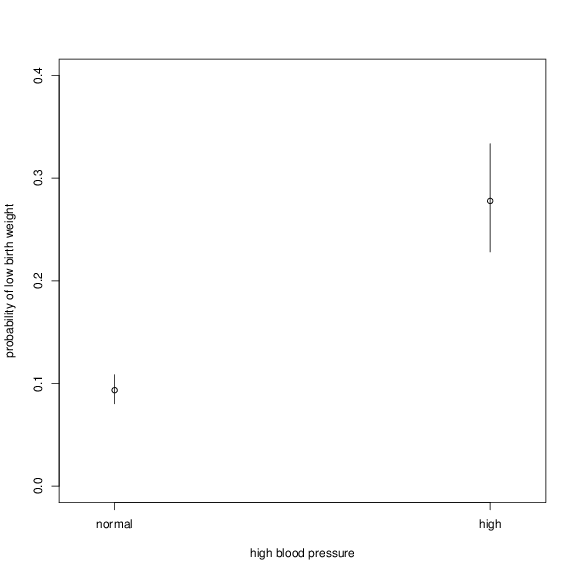
\includegraphics[width=6.5cm]{effect1.png}
\end{center}
\end{itemize}
\end{frame}

\begin{frame}[fragile]\frametitle{Understanding the Coefficients}
\begin{itemize}
\item and one effect plot (\texttt{effects} package)
  \begin{exampleblock}{Input}
\begin{verbatim}
> plot(Effect("hyp",m))
\end{verbatim}
  \end{exampleblock}
\begin{center}
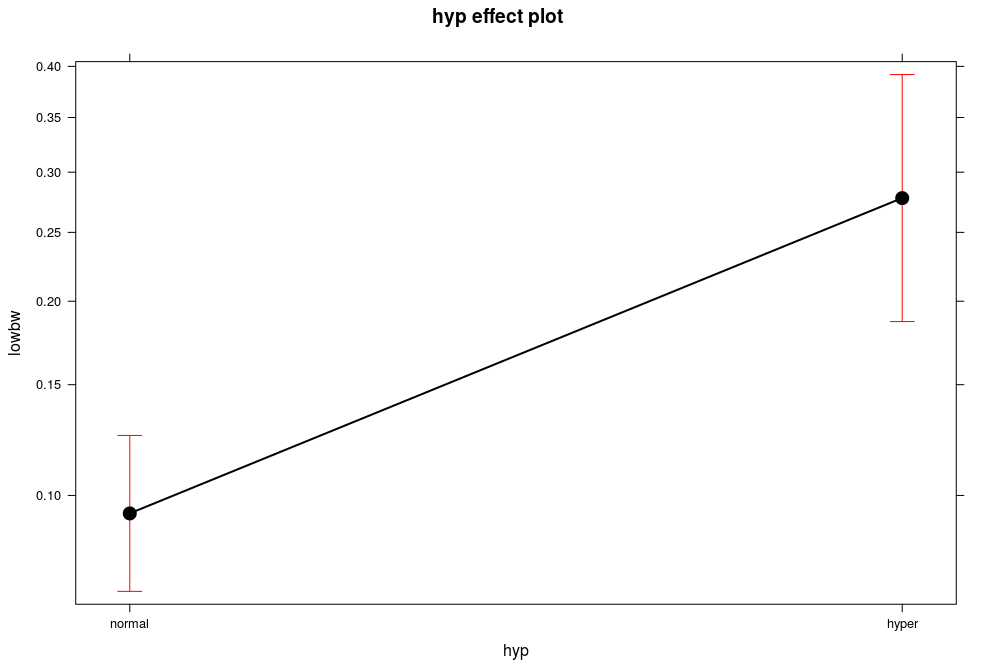
\includegraphics[width=10cm]{effect2.png}
\end{center}
\end{itemize}
\end{frame}


\begin{frame}[fragile]\frametitle{Understanding the Coefficients}
\begin{itemize}
\item btw: \texttt{Effect()} gives you the probabilities without using a explicit transformation
  \begin{exampleblock}{Input/Output}
\begin{verbatim}
> Effect("hyp",m)

 hyp effect
hyp
    normal      hyper 
0.09345794 0.27777778 
\end{verbatim}
  \end{exampleblock}
\end{itemize}
\end{frame}


\begin{frame}[fragile]\frametitle{Controlling}
Controlling the effect of \texttt{hyp} on \texttt{lowbw} for \texttt{sex}\footnotesize
\begin{exampleblock}{Input/Output}
\begin{verbatim}
> m2 <- glm(lowbw ~ hyp+sex, family=binomial, data=births)

            Estimate   StdErr  Pr(>|z|)    
(Intercept)  -2.5088   0.2331  < 2e-16 ***
hyphyper      1.3625   0.3144 1.47e-05 *** hyp controlled for sex
sexF          0.4473   0.2843    0.116     sex controlled for hyp
\end{verbatim}
\end{exampleblock}
\normalsize
When you control for a variable you are assuming that any interaction can be ignored.
\end{frame}


\begin{frame}[fragile]\frametitle{Interaction (effect modification)}
\begin{itemize}
\item We add an interaction term to the model\small
  \begin{exampleblock}{Input/Output}
\begin{verbatim}
> m3 <- glm(lowbw ~ hyp + sex + hyp:sex, 
+           family=binomial, data=births) # or shorter
> m3 <- glm(lowbw ~ hyp*sex, family=binomial, 
            data=births)
\end{verbatim}
  \end{exampleblock}
\end{itemize}
\end{frame}

\begin{frame}[fragile]\frametitle{Interaction (effect modification)}
\begin{itemize}
\item we have four estimates now, and to get the effects in terms of probabilites we need to type\scriptsize
  \begin{exampleblock}{Input/Output}
\begin{verbatim}
> m3 <- glm(lowbw ~ hyp*sex, family=binomial, data=births)
> summary(m3)

Call:
glm(formula = lowbw ~ hyp * sex, family = binomial, data = births)

Deviance Residuals: 
    Min       1Q   Median       3Q      Max  
-0.8090  -0.5074  -0.3749  -0.3749   2.3195  

Coefficients:
              Estimate Std. Error z value Pr(>|z|)    
(Intercept)    -2.6198     0.2674  -9.796  < 2e-16 ***
hyphyper        1.6707     0.4326   3.862 0.000112 ***
sexF            0.6347     0.3421   1.855 0.063535 .  
hyphyper:sexF  -0.6507     0.6366  -1.022 0.306694    
---
Signif. codes:  0 ‘***’ 0.001 ‘**’ 0.01 ‘*’ 0.05 ‘.’ 0.1 ‘ ’ 1

(Dispersion parameter for binomial family taken to be 1)

    Null deviance: 366.92  on 499  degrees of freedom
Residual deviance: 347.29  on 496  degrees of freedom
AIC: 355.29

Number of Fisher Scoring iterations: 5
\end{verbatim}
  \end{exampleblock}
\end{itemize}
\end{frame}


\begin{frame}[fragile]\frametitle{Interaction Coefficients}
  \begin{exampleblock}{Input/Output}\scriptsize
\begin{verbatim}
> invlogit(coef(m3)[1])
  (Intercept) 
   0.0678733 
> invlogit(coef(m3)[1] + coef(m3)[2])
  (Intercept) 
   0.2790698 
> invlogit(coef(m3)[1] + coef(m3)[3])
  (Intercept) 
   0.1207729 
> invlogit(coef(m3)[1] + coef(m3)[2] + coef(m3)[3] + coef(m3)[4])
  (Intercept) 
   0.2758621 
\end{verbatim}
  \end{exampleblock}
\end{frame}

\begin{frame}[fragile]\frametitle{Exercises}
You can calculate the effects by hand and using the \texttt{invlogit()} function, but this becomes a little annoying, the \texttt{allEffects()} function provides a nicer way to do the same.
\begin{itemize}
\item now you have three models, use the \texttt{Effects()}, \texttt{allEffects()} and the \texttt{plot()} function to get the following information:
  \begin{enumerate}
  \item the estimated probability for moms with hypertension to get a baby with low birth weight for all three models
  \item is their a difference in effects between boys and girls? Which model can answer this question?
  \end{enumerate}
\end{itemize}
\end{frame}


\begin{frame}[fragile]\frametitle{Testing for Interaction}
\begin{itemize}
\item Do we need to keep the interaction term? \footnotesize
  \begin{exampleblock}{Input/Output}
\begin{verbatim}
> m2 <- glm(lowbw ~ hyp+sex, family=binomial, 
+                            data=births)
> m3 <- glm(lowbw ~ hyp*sex, family=binomial, 
+                            data=births)
> anova(m2,m3,test="Chisq")

  Resid. Df Resid. Dev Df Deviance Pr(>Chi)
1       497     348.34                     
2       496     347.29  1   1.0561   0.3041
\end{verbatim}
  \end{exampleblock}
\normalsize
\item The \texttt{anova} function conducts an \emph{analysis of variance} -- a test of significance between two nested models. 
\item The interaction term does not improve the fit - so we leave it out and keep the simpler model.
\end{itemize}
\end{frame}


\begin{frame}[fragile]\frametitle{Stratified Effects}
\begin{itemize}
\item When there is a strong interaction it may be best to report stratified effects. 
\item Omitting the main effect of \texttt{hyp} in an interaction model gives us the effect of \texttt{hyp} within strata of \texttt{sex}.\scriptsize
\end{itemize}
\end{frame}

\begin{frame}[fragile]\frametitle{Stratified Effects}
  \begin{exampleblock}{Input/Output}\footnotesize
\begin{verbatim}
> m4 <- glm(lowbw ~ sex + sex:hyp, family=binomial, data=births)
> summary(m4)

Call:
glm(formula = lowbw ~ sex + sex:hyp, family = binomial, data = births)

Deviance Residuals: 
    Min       1Q   Median       3Q      Max  
-0.8090  -0.5074  -0.3749  -0.3749   2.3195  

Coefficients:
              Estimate Std. Error z value Pr(>|z|)    
(Intercept)    -2.6198     0.2674  -9.796  < 2e-16 ***
sexF            0.6347     0.3421   1.855 0.063535 .  
sexM:hyphyper   1.6707     0.4326   3.862 0.000112 ***
sexF:hyphyper   1.0200     0.4670   2.184 0.028952 *  
---
Signif. codes:  0 ‘***’ 0.001 ‘**’ 0.01 ‘*’ 0.05 ‘.’ 0.1 ‘ ’ 1

(Dispersion parameter for binomial family taken to be 1)

    Null deviance: 366.92  on 499  degrees of freedom
Residual deviance: 347.29  on 496  degrees of freedom
AIC: 355.29

Number of Fisher Scoring iterations: 5
\end{verbatim}
  \end{exampleblock}
\end{frame}


\begin{frame}[fragile]\frametitle{Stratified Effects}
A slightly shorter way to define the same model:
  \begin{exampleblock}{Input/Output}\footnotesize
\begin{verbatim}
> m4 <- glm(lowbw ~ sex/hyp, family=binomial, data=births)
> m4

Call:  glm(formula = lowbw ~ sex/hyp, family = binomial, data = births)

Coefficients:
  (Intercept)           sexF  sexM:hyphyper  sexF:hyphyper  
      -2.6198         0.6347         1.6707         1.0200  

Degrees of Freedom: 499 Total (i.e. Null);  496 Residual
Null Deviance:	    366.9 
Residual Deviance: 347.3 	AIC: 355.3
\end{verbatim}
  \end{exampleblock}
\end{frame}


\begin{frame}[fragile]\frametitle{Exercise}
\begin{itemize}
\item compare the effects in \texttt{m3} and \texttt{m4}
\end{itemize}
\end{frame}

\begin{frame}[fragile]\frametitle{Understanding the Coefficients}
    \begin{columns}\small
      \begin{column}{0.5\textwidth}
\begin{verbatim}
> ftable(births$hyp,
+        births$sex,
+        births$lowbw)
          normal low
                    
normal M     206  15
       F     182  25
hyper  M      31  12
       F      21   8
\end{verbatim}
      \end{column}
      \begin{column}{0.5\textwidth}
\begin{verbatim}
## male/normal bp
> 15/(206+15)
[1] 0.0678733
## female/normal bp
> 25/(25+182)
[1] 0.1207729
## male/high bp
> 12/(12+31)
[1] 0.2790698
## female/high bp
> 8/(8+21)
[1] 0.2758621
\end{verbatim}
      \end{column}
    \end{columns}
\end{frame}

\subsection{Binomial/Logistic Regression}

\begin{frame}[fragile]\frametitle{Simple Logistic Regression}
\begin{itemize}
\item now we model the probability of low birth weight dependent on gestational age
\item so the model in R is 
  \begin{exampleblock}{Input}\footnotesize
\begin{verbatim}
> m5 <- glm(lowbw ~ gestwks, family=binomial, data=births)
\end{verbatim}
  \end{exampleblock}\normalsize
\item and as math formula
$$ \log\left(\frac{\mbox{Pr(lowbw)}}{1-\mbox{Pr(lowbw)}}\right) = \beta_0 + \beta_1 \cdot \mbox{gestwks} + \epsilon$$
\end{itemize}
\end{frame}


\begin{frame}[fragile]\frametitle{Simple Logistic Regression}
\begin{itemize}
\item where the output look similar to the output above
  \begin{exampleblock}{Input/Output}\scriptsize
\begin{verbatim}
> summary(m5)

Call:
glm(formula = lowbw ~ gestwks, family = binomial, data = births)

Deviance Residuals: 
    Min       1Q   Median       3Q      Max  
-2.0873  -0.3623  -0.2223  -0.1369   2.9753  

Coefficients:
            Estimate Std. Error z value Pr(>|z|)    
(Intercept)  31.8477     4.0574   7.849 4.18e-15 ***
gestwks      -0.8965     0.1084  -8.272  < 2e-16 ***
---
Signif. codes:  0 ‘***’ 0.001 ‘**’ 0.01 ‘*’ 0.05 ‘.’ 0.1 ‘ ’ 1

(Dispersion parameter for binomial family taken to be 1)

    Null deviance: 360.38  on 489  degrees of freedom
Residual deviance: 205.75  on 488  degrees of freedom
  (10 observations deleted due to missingness)
AIC: 209.75

Number of Fisher Scoring iterations: 6
> m5 <- glm(lowbw ~ gestwks, family=binomial, data=births)
\end{verbatim}
  \end{exampleblock}
\end{itemize}
\end{frame}


\begin{frame}[fragile]\frametitle{Understanding the Coefficients}
\begin{itemize}
\item this relationship is described by $$\mbox{Pr(lowbw)}=\mbox{logit}^{-1}(31.8477 + -0.8965 \cdot \mbox{gestwks}) $$
\item the intercept
  \begin{exampleblock}{Input/Output}
\begin{verbatim}
> invlogit(coef(m)[1])
(Intercept) 
  1
\end{verbatim}
  \end{exampleblock}
is interpretable as the probability for a low birth weight at a hypothetical gestational age of 0 (which makes no sense because it lies outside the range of gestational ages in our data)
\item the parameter for \texttt{gestwks} describes how fast the probability decreases with increasing gestation age
\end{itemize}
\end{frame}

\begin{frame}[fragile]\frametitle{Understanding the Coefficients}
$$\mbox{Pr(lowbw)}=\mbox{logit}^{-1}(31.8477 + -0.8965 \cdot \mbox{gestwks}) $$
\begin{itemize}
\item the coefficient for \texttt{gestwks} is best interpretable if we use it as argument to the exponential function
  \begin{exampleblock}{Input/Output}
\begin{verbatim}
> exp(coef(m5)[2])
  gestwks 
0.4080114 
\end{verbatim}
  \end{exampleblock}
this way it is interpretable as odds ratio for low birth weight for a difference of 1 week of gestational age
\end{itemize}
\end{frame}


\begin{frame}[fragile]\frametitle{Exercise}
  \begin{enumerate}
  \item here is a example for the \texttt{Effects()} command for regression
    \begin{exampleblock}{Input/Output}\scriptsize
\begin{verbatim}
> Effect("gestwks",m5)

 gestwks effect
gestwks
        25         30         35         40 
0.99992022 0.99299324 0.61574996 0.01779725 
> Effect("gestwks",m5,xlevels = list(gestwks = c(20,30,40)))

 gestwks effect
gestwks
        20         30         40 
0.99999910 0.99299324 0.01779725   
\end{verbatim}
    \end{exampleblock}\normalsize
\item use the command to gain the estimated probability of low birth weight for a gestational age of 27 and 36 weeks
  \end{enumerate}
\end{frame}


\begin{frame}[fragile]\frametitle{\texttt{ggplot()} and \texttt{glm()}}
  \begin{itemize}
  \item ggplot2 knows also glms
  \item unfortunately the y-variable needs to be coded in 0s and 1s, but we can do this on the fly with \texttt{as.numeric()}
  \end{itemize}
  \begin{exampleblock}{Input}\scriptsize
\begin{verbatim}
> require(ggplot2)
> ggplot(births,aes(x = gestwks, y = as.numeric(lowbw)-1)) +
+     geom_smooth(method = "glm", family = "binomial",se = F,size = 2) +
+     geom_point(shape="|")  ## adds actual values  
\end{verbatim}
  \end{exampleblock}
\end{frame}


\begin{frame}\frametitle{\texttt{ggplot()} and \texttt{glm()}}
  \begin{center}
    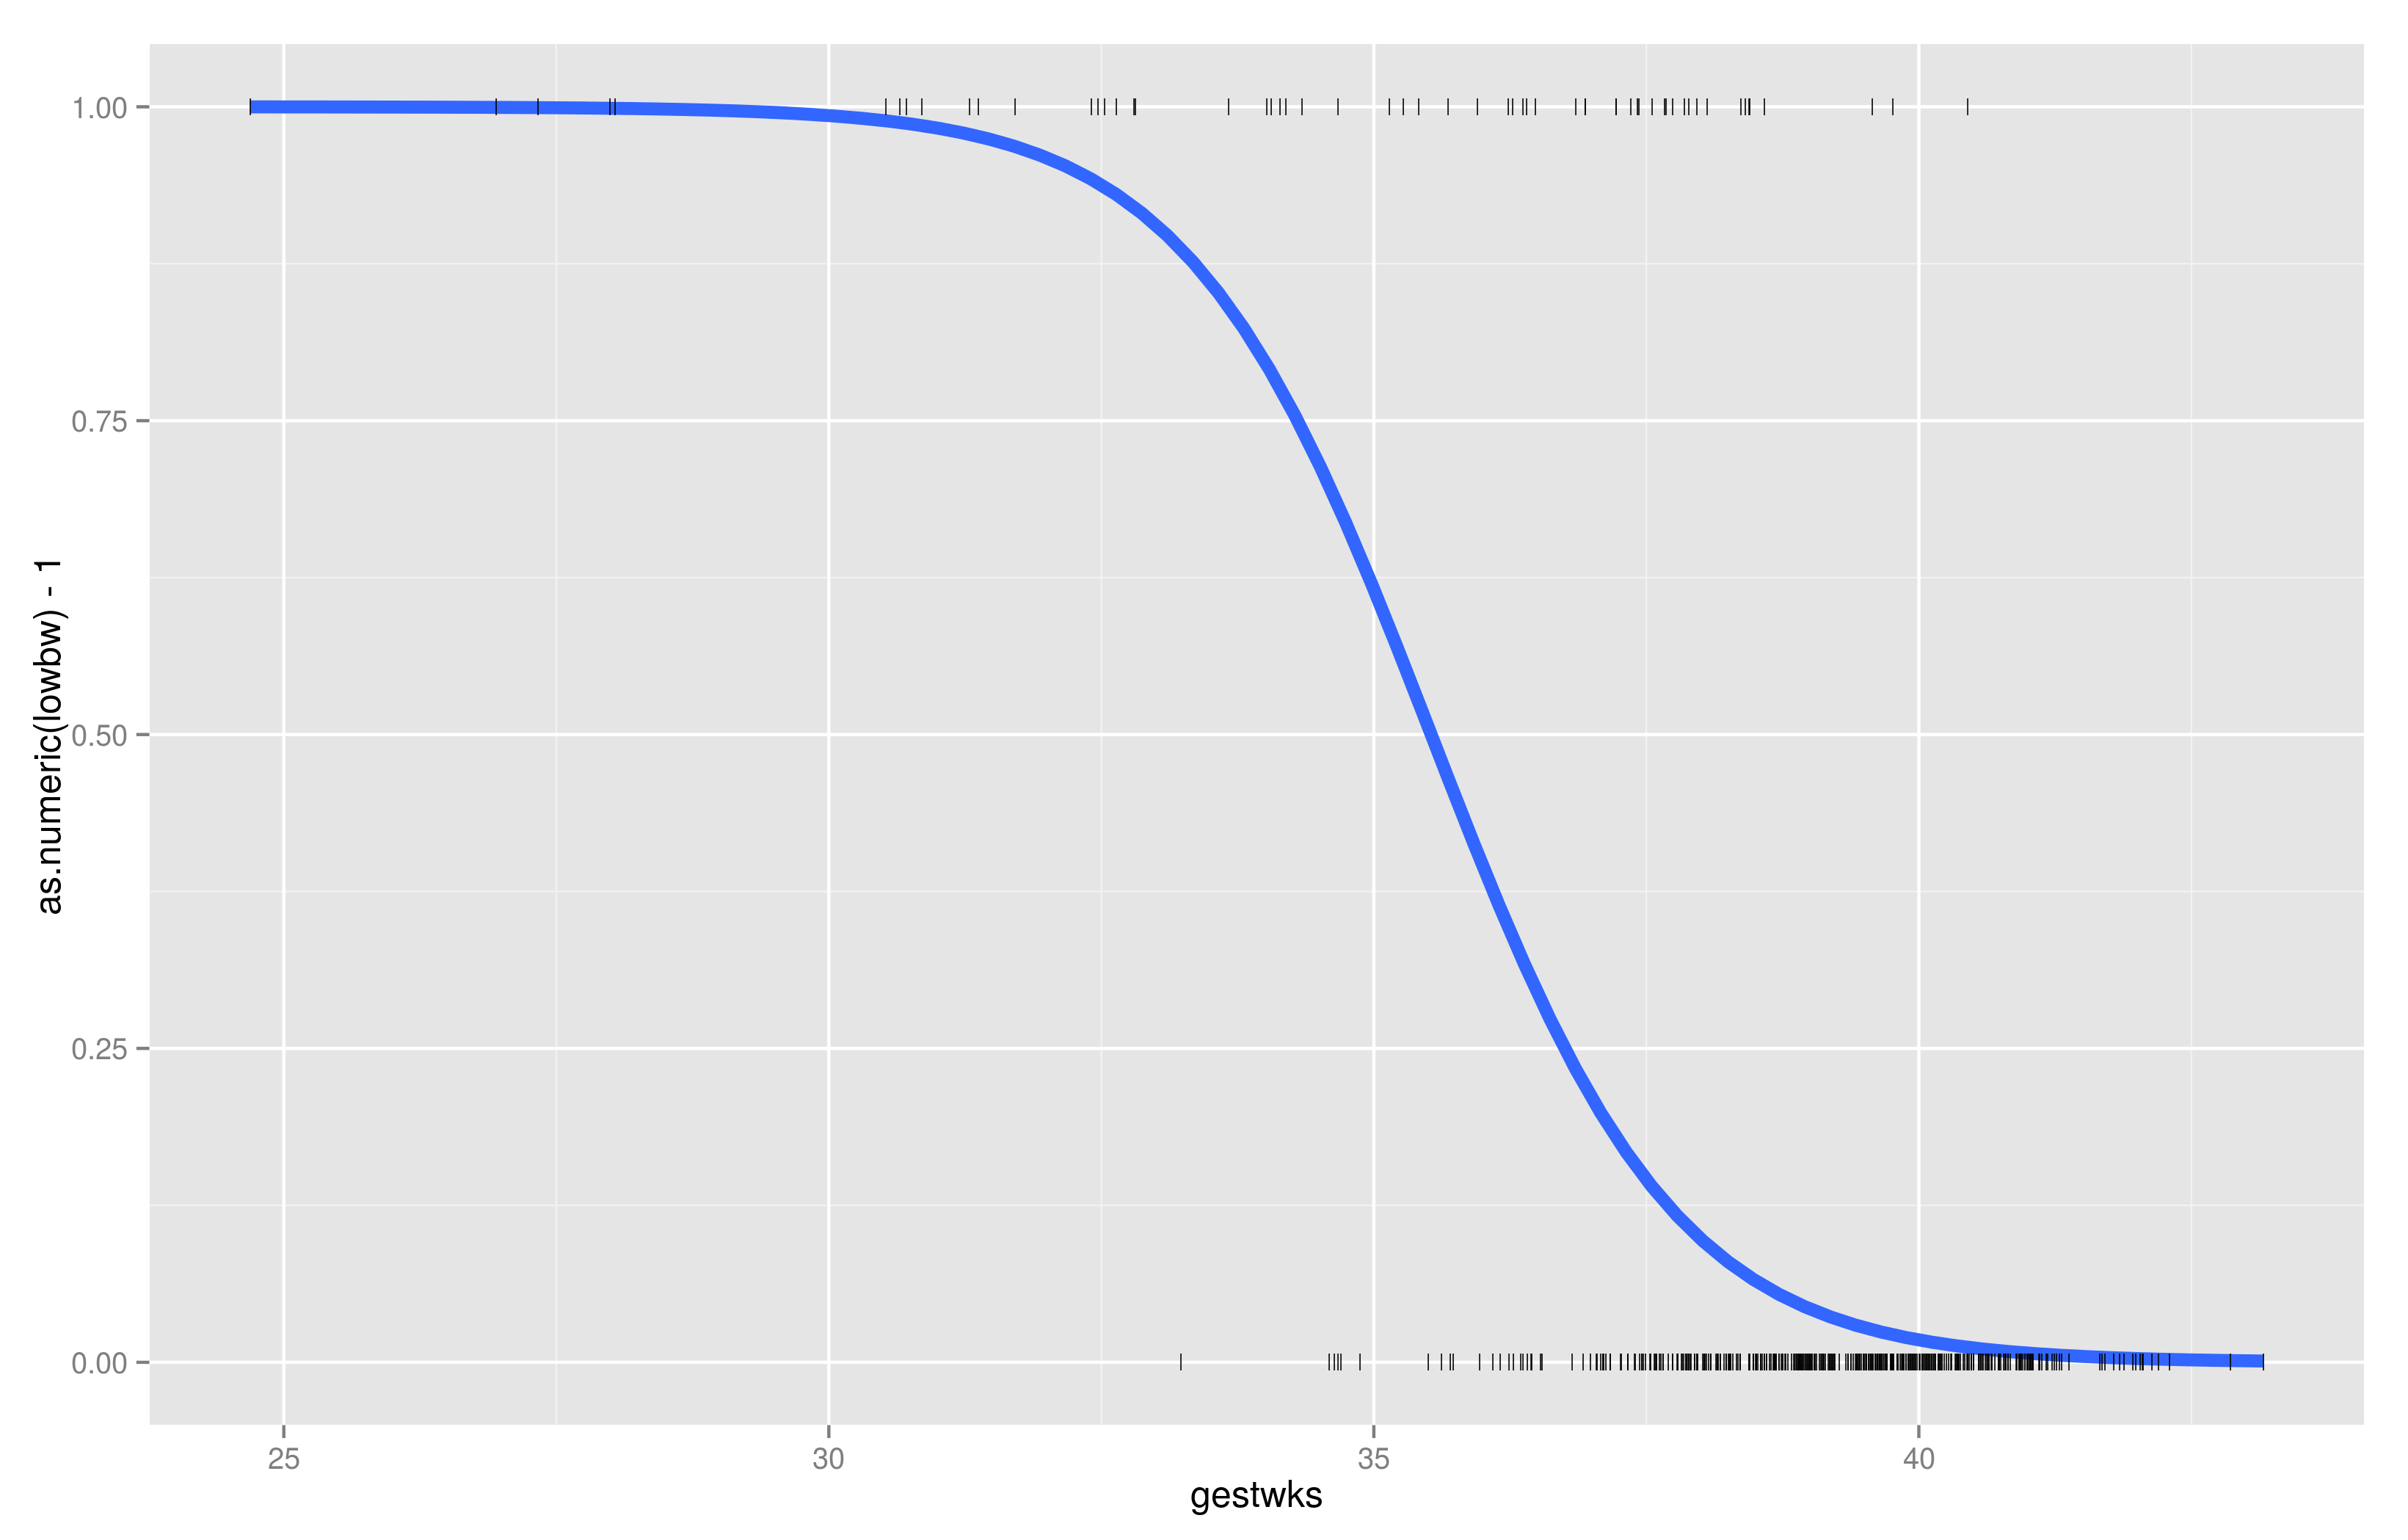
\includegraphics[width=11cm]{glmggplot.png}
  \end{center}
\end{frame}


\begin{frame}[fragile]\frametitle{Exercise}
Take the code producing the graph
  \begin{enumerate}
  \item try to change the axis titles (\texttt{xlab()} and \texttt{ylab()})
  \item add a title (\texttt{ggtitle()})
  \item change the colour of the function to black, set se = T
  \item change the colour of the points to red for the low birth weight and green for the one with normal birth weight
  \item change the position of the legend; place it somewhere near the upper right corner inside the plotting area (\texttt{legend.position})
  \end{enumerate}
\end{frame}

\subsection{The famous O-Ring example}

\begin{frame}[fragile]\frametitle{The Challenger Disaster Example}
In January 1986, the space shuttle Challenger exploded shortly after launch. An
investigation was launched into the cause of the crash and attention focused on the rubber
O-ring seals in the rocket boosters. At lower temperatures, rubber becomes more brittle
and is a less effective sealant. At the time of the launch, the temperature was 31\degree F. Could
the failure of the O-rings have been predicted? In the 23 previous shuttle missions for
which data exists, some evidence of damage due to blow by and erosion was recorded on
some O-rings. Each shuttle had two boosters, each with three O-rings. For each mission,
we know the number of O-rings out of six showing some damage and the launch
temperature.(faraway)
\end{frame}

\begin{frame}[fragile]\frametitle{The Challenger Disaster Example}
\begin{itemize}
\item the data are given in the data frame \texttt{orings} in the \texttt{faraway} package
\item after loading we have a look at the first six lines
\begin{verbatim}
> library(faraway)
> data(orings)
> head(orings)
  temp damage
1   53      5
2   57      1
3   58      1
4   63      1
5   66      0
6   67      0
\end{verbatim}
\item we see that every shuttle mission has its own row (but not every O-ring)
\end{itemize}
\end{frame}

\begin{frame}[fragile]\frametitle{The Challenger Disaster Example}
\begin{itemize}
\item that is not a problem: one way of defining a binary response variable in a glm is to form a two-column matrix with the first
column representing the number of “successes” y and the second column the number of “failures” n–y.
\begin{verbatim}
> m <- glm(cbind(damage,6-damage) ~ temp,
+                      family=binomial, orings)
\end{verbatim}
\normalsize
\item we see that every shuttle mission has its own row (but not every O-ring)
\end{itemize}
\end{frame}

\begin{frame}[fragile]\frametitle{The Challenger Disaster Example}
\begin{itemize}
\item the output looks familiar:\footnotesize
\begin{verbatim}
> summary(m)
Call:
glm(formula = cbind(damage, 6 - damage) ~ temp, 
     family = binomial, data = orings)
Deviance Residuals: 
    Min       1Q   Median       3Q      Max  
-0.9529  -0.7345  -0.4393  -0.2079   1.9565  
Coefficients:
            Estimate Std. Error z value Pr(>|z|)    
(Intercept) 11.66299    3.29626   3.538 0.000403 ***
temp        -0.21623    0.05318  -4.066 4.78e-05 ***
(Dispersion parameter for binomial family taken to be 1)
    Null deviance: 38.898  on 22  degrees of freedom
Residual deviance: 16.912  on 21  degrees of freedom
AIC: 33.675
\end{verbatim}
\item remember, the response is a probability. Therefore our model describes the probability of a damaged O-ring depending on the temperature
\end{itemize}
\end{frame}


\begin{frame}[fragile]\frametitle{Understanding the Coefficients}
\begin{itemize}
\item this relationship is described by $$\mbox{Pr(damage)}=\mbox{logit}^{-1}(11.66299 + -0.21623 \cdot \mbox{temp}) $$
\item the intercept
\begin{verbatim}
> invlogit(coef(m)[1])
(Intercept) 
  0.9999914 
\end{verbatim}
is interpretable as the probability for a damaged O-ring at a temperature of 0\degree F
\item the parameter for temperature describes how fast the probability decreases with increasing temperature
\end{itemize}
\end{frame}

\begin{frame}[fragile]\frametitle{Understanding the Coefficients}\footnotesize
\begin{verbatim}
> tf <- 20:100
> pd <- predict(m,newdata=list(temp=tf), type="response")
> plot(tf,pd,type="l",
+  xlab=expression(paste("temperature (",degree,"F)",sep=" ")),
+  ylab="probability of damage")
\end{verbatim}
\begin{center}
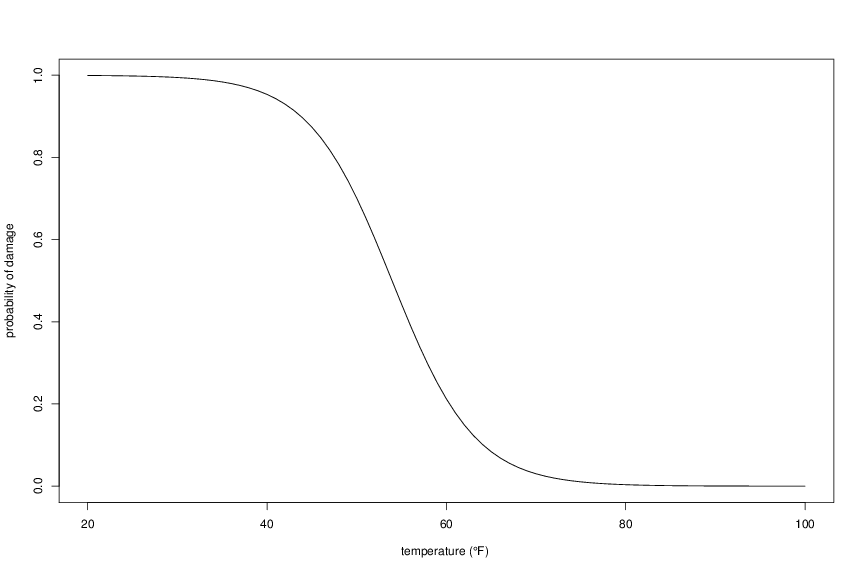
\includegraphics[width=7cm]{challenger.png}
\end{center}
\end{frame}

\begin{frame}[fragile]\frametitle{Understanding the Coefficients}
and the same plot made with ggplot (incl. adding a table)
\begin{center}
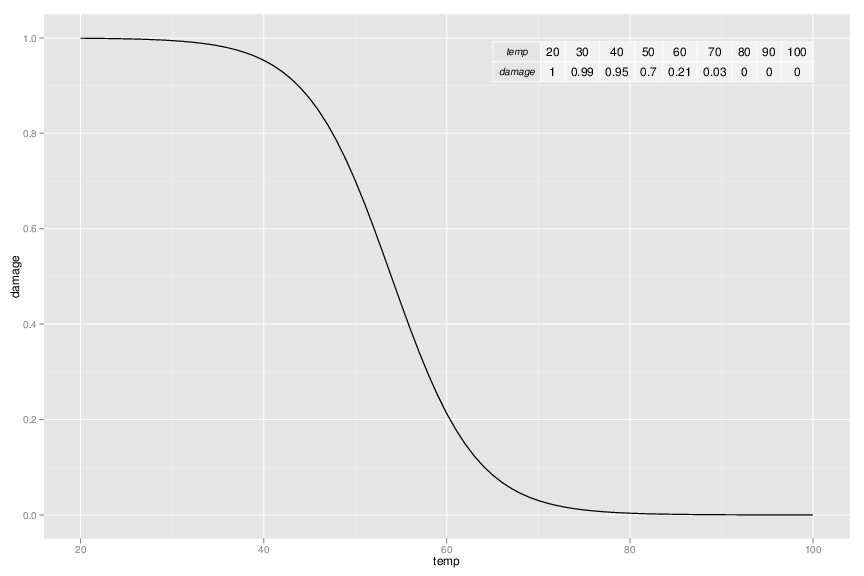
\includegraphics[width=7cm]{challenger2.png}
\end{center}
\end{frame}

\subsection[Binomial Ancova]{Ancova with a Binary Response Variable }

\begin{frame}[fragile]\frametitle{Parasite Infection Example}
\begin{itemize}
\item the binary response variable is parasite infection (infected or not) 
\item the explanatory variables are weight and age (continuous) 
\item and sex (categorical)
\item we want to investigate if there is a different effect of age for each of the sexes on the outcome variable
\end{itemize}
\begin{verbatim}
> infection <- read.table("infection.txt",header=T)
> summary(infection)
    infected          age              sex       
 Min.   :0.000   Min.   :  2.00   Min.   :0.000  
 1st Qu.:0.000   1st Qu.: 46.00   1st Qu.:0.000  
 Median :0.000   Median : 84.50   Median :1.000  
 Mean   :0.324   Mean   : 93.69   Mean   :0.514  
 3rd Qu.:1.000   3rd Qu.:139.25   3rd Qu.:1.000  
 Max.   :1.000   Max.   :200.00   Max.   :1.000  
\end{verbatim}
\end{frame}


\begin{frame}[fragile]\frametitle{Parasite Infection Example}\footnotesize
\begin{verbatim}
> m <- glm(infected~age*sex,family=binomial,
+                               data=infection)
> summary(m)
Call:
glm(formula = infected ~ age * sex, family = binomial, 
                                     data = infection)
Deviance Residuals: 
    Min       1Q   Median       3Q      Max  
-2.0411  -0.7307  -0.4363   0.6632   2.3215  
Coefficients:
             Estimate Std. Error z value Pr(>|z|)    
(Intercept) -3.000513   0.413639  -7.254 4.05e-13 ***
age          0.015657   0.003176   4.929 8.25e-07 ***
sex          0.116664   0.553956   0.211   0.8332    
age:sex      0.011050   0.004612   2.396   0.0166 *  

(Dispersion parameter for binomial family taken to be 1)
    Null deviance: 629.85  on 499  degrees of freedom
Residual deviance: 477.61  on 496  degrees of freedom
AIC: 485.61
\end{verbatim}
\end{frame}

\begin{frame}[fragile]\frametitle{Parasite Infection Example}
\begin{itemize}
\item so for male at a age of 0 there is a probability of
\begin{verbatim}
> invlogit(coef(m)[1])
(Intercept) 
 0.04740269 
\end{verbatim}
\item for females is the probability at age 0 
\begin{verbatim}
> invlogit(coef(m)[1]+coef(m)[3])
(Intercept) 
 0.05295775 
\end{verbatim}
\end{itemize}
\end{frame}


\begin{frame}[fragile]\frametitle{Parasite Infection Example}
\begin{itemize}
\item so what about the slope?
\item for males the underlying model is the following
$$\mbox{Pr(infection)}=\mbox{logit}^{-1}(-3.000513 + 0.015657 \cdot \mbox{age}) $$
\item for females the slope is almost twice as high
$$\mbox{Pr(infection)}=\mbox{logit}^{-1}(-2.883849 + 0.02670685  \cdot \mbox{age}) $$
\item we can compare them by looking at the age where the probability to be infected is 50\%
\end{itemize}
\end{frame}

\begin{frame}[fragile]\frametitle{Parasite Infection Example}
\begin{itemize}
\item this is the case when $-3.000513 + 0.015657 \cdot \mbox{age}=0$  respectively $-2.883849 + 0.02670685  \cdot \mbox{age}=0$; you can do it by hand or use R\small
\begin{verbatim}
> ## male
> solve(0.015657,3.000513)
[1] 191.6404
> ## female
> solve(0.02670685,2.883849,)
[1] 107.9816
\end{verbatim}
\normalsize
\item \texttt{solve()} solves systems of linear equations in the form A*x=b, where A is the matrix of coefficients and b are the (negative) intercepts, here we have the special case with just one equation
\end{itemize}
\end{frame}

\begin{frame}[fragile]\frametitle{Parasite Infection Example}
\begin{itemize}
\item you can also use the \texttt{allEffects()} function (part of the \texttt{effects} package), which give you the probabilities for being infected on several ages for both sexes\footnotesize
\begin{verbatim}
> allEffects(m)
 model: infected ~ age * sex

 age*sex effect
     sex
age            0          1
  2   0.04883687 0.05570148
  24  0.06756215 0.09596497
  46  0.09276694 0.16038932
  68  0.12610300 0.25582483
  90  0.16918450 0.38219715
  112 0.22322468 0.52680374
  134 0.28853152 0.66704908
  156 0.36399154 0.78286130
  178 0.44679328 0.86645480
  200 0.53265591 0.92110968
\end{verbatim}
\end{itemize}
\end{frame}


\begin{frame}[fragile]\frametitle{Parasite Infection Example}
\begin{center}
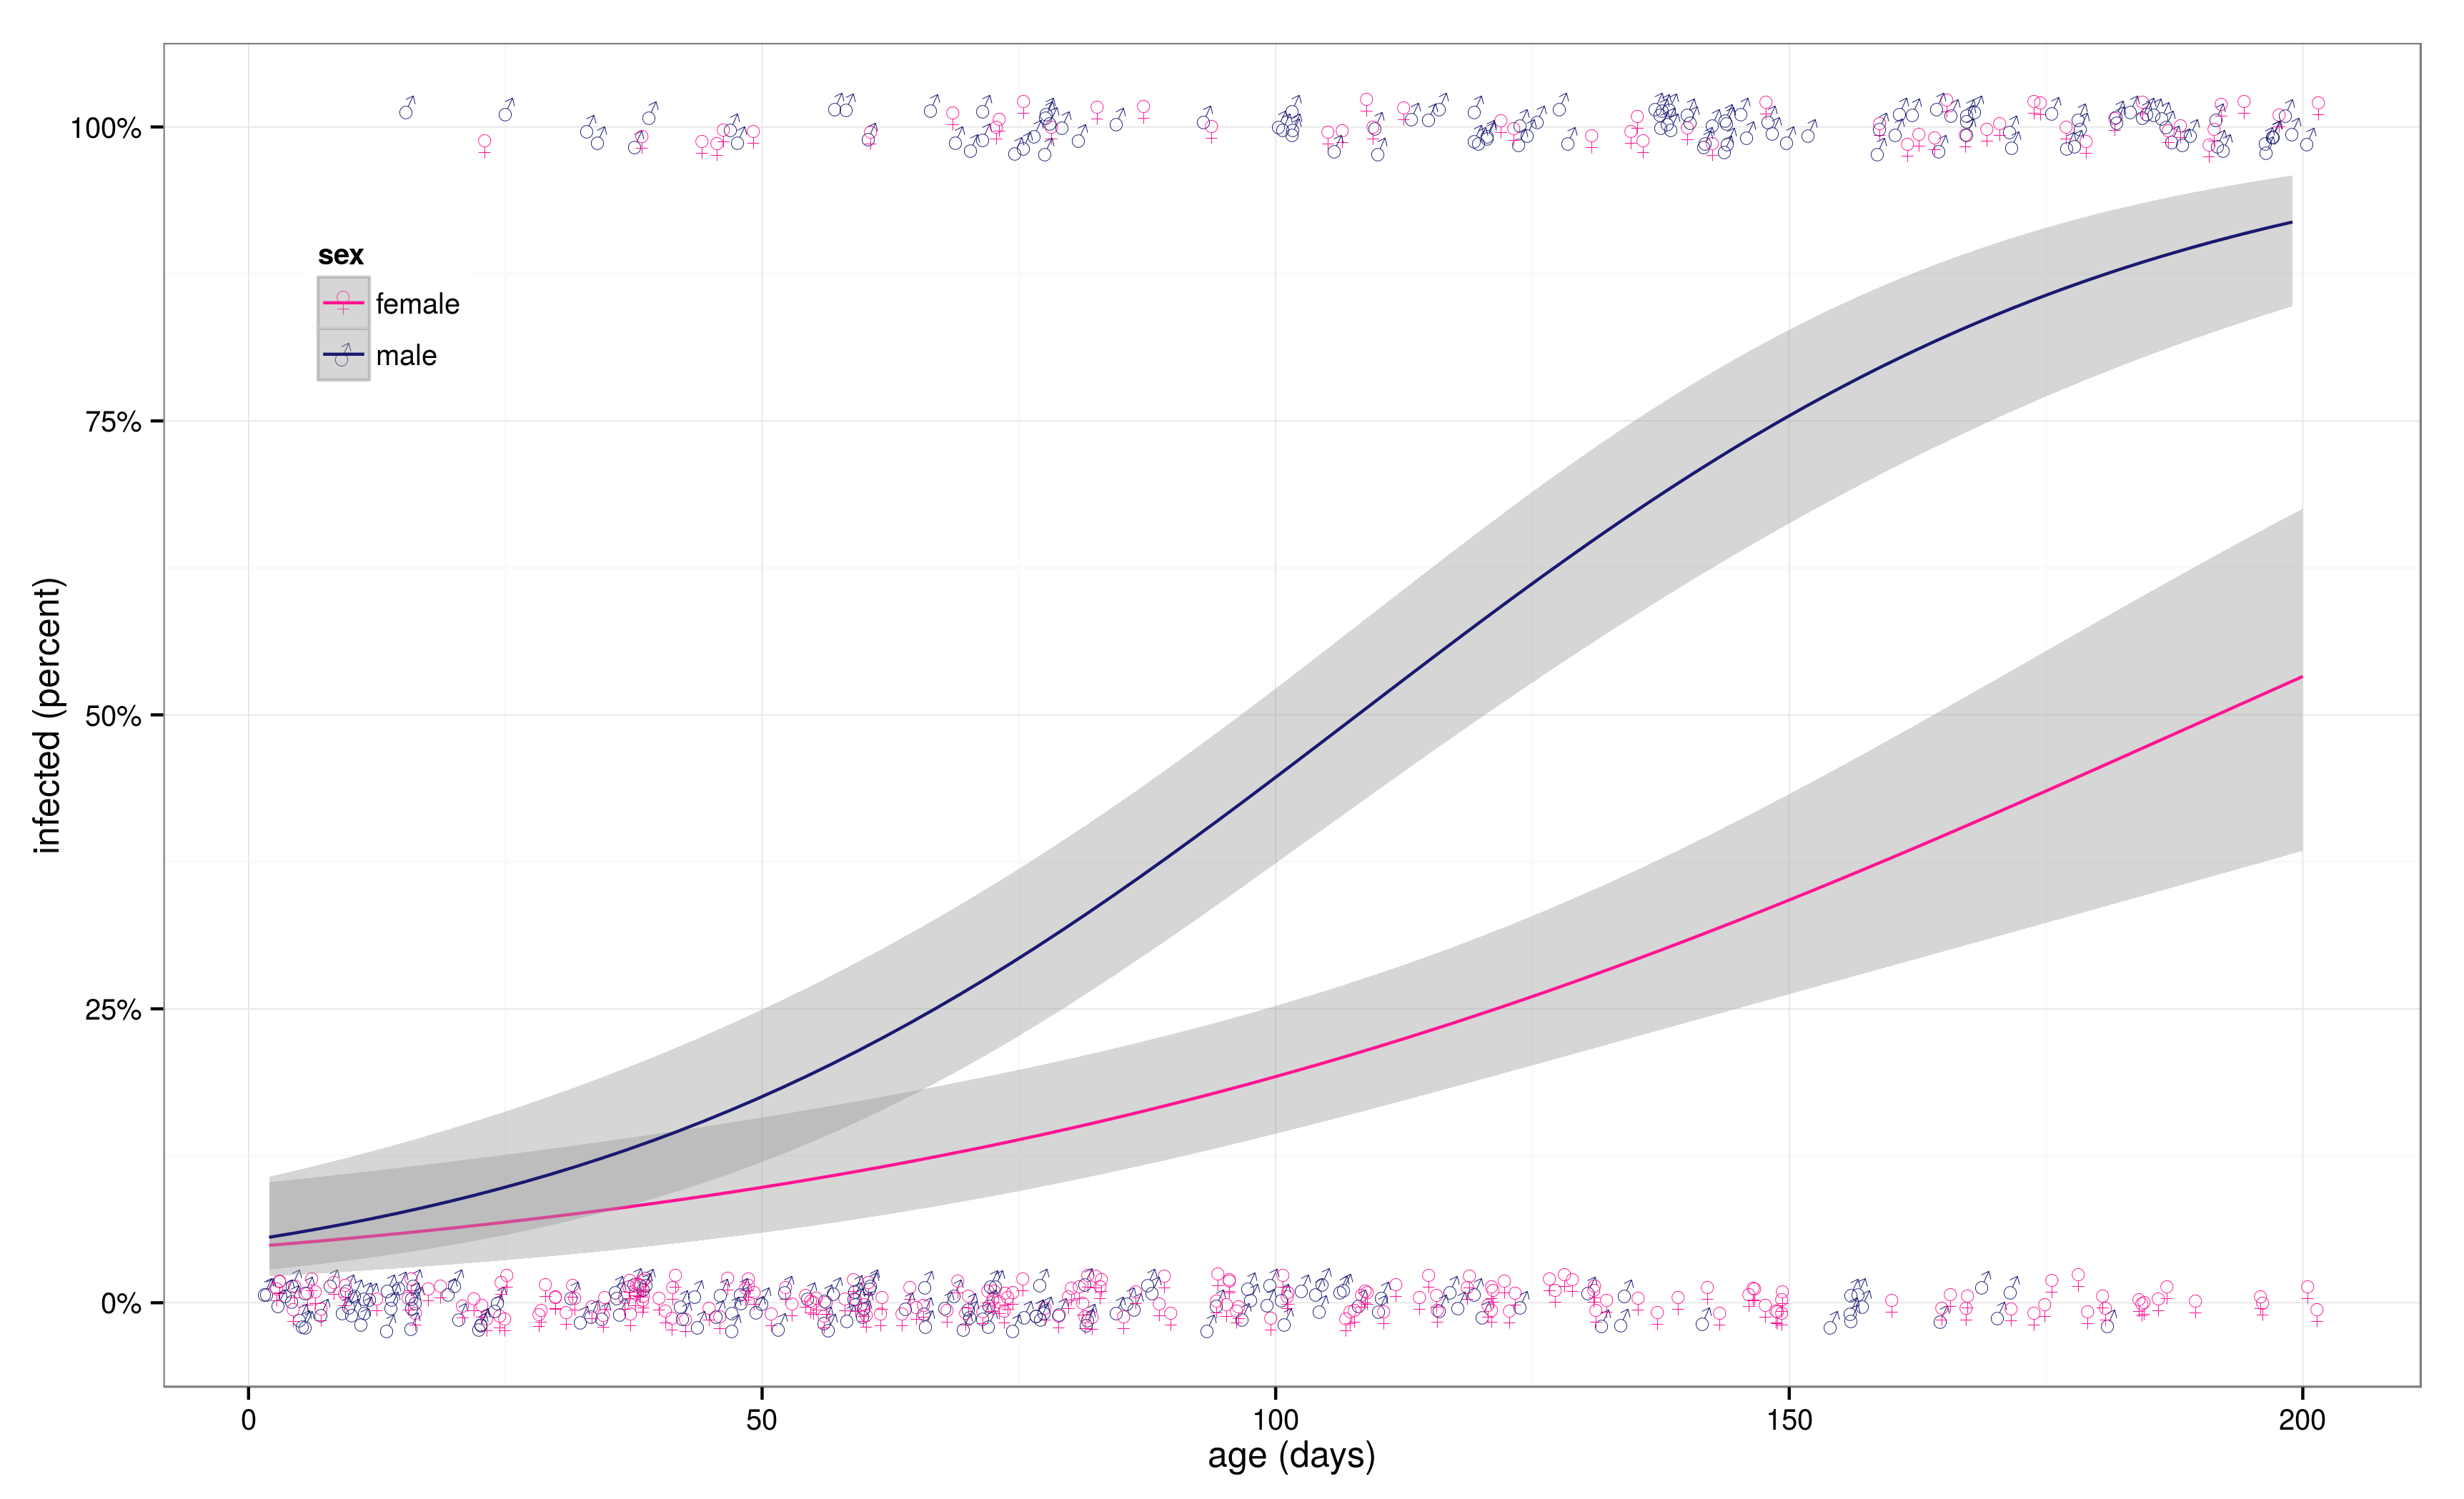
\includegraphics[width=7cm]{binancova1.png}
\end{center}
\end{frame}

\section{GLMs and Count Data}

\begin{frame}[fragile]\frametitle{Count Data}
\begin{itemize}
\item a great deal of the data collected is in the form of counts
\item for example:
  \begin{itemize}
  \item number of individuals that died
  \item number of firms going
  \item bankrupt, the number of days of frost, 
  \item the number of red blood cells on a microscope slide, and the 
  \item number of craters in a sector of lunar landscape
  \end{itemize}
\item with count data, the number 0 often appears as a value of the response (zero inflated data)
\end{itemize}
\end{frame}

\begin{frame}[fragile]\frametitle{Count Data}
\begin{itemize}
\item we must consider a different cases in dealing with data on frequencies: cases
  \begin{itemize}
  \item   where we count how many
times something happened, but we have no way of knowing how often it did not happen
(e.g. lightning strikes, bankruptcies, deaths, births). 
\item count data on proportions, where we know the number doing a particular thing, but also the number
not doing that thing (e.g. the proportion dying, sex ratios at birth, proportions of different
groups responding to a questionnaire)
  \end{itemize}
\end{itemize}
\end{frame}

\begin{frame}[fragile]\frametitle{A Poisson Regression}
  \begin{itemize}
  \item The following example has a count (the number of reported cancer cases per year per clinic) as the response variable
  \item and a single continuous explanatory variable (the distance from a nuclear plant to the clinic in km). 
  \item The question is whether or not proximity to the reactor affects the number of cancer cases.\small
\begin{verbatim}
> cancer <- read.table("clusters.txt",header=T)
> head(cancer)
  Cancers Distance
1       0 11.46952
2       0 66.55395
3       0 47.46230
4       0 48.38129
5       0 73.76534
6       0 70.57555
\end{verbatim}
  \end{itemize}
\end{frame}


\begin{frame}[fragile]\frametitle{Count Data}
  \begin{itemize}
  \item look at a barplot (cut the \texttt{Distance} variable in ten classes) and a scatter plot
  \end{itemize}
  \begin{columns}
    \begin{column}{0.5\textwidth}
\begin{center}
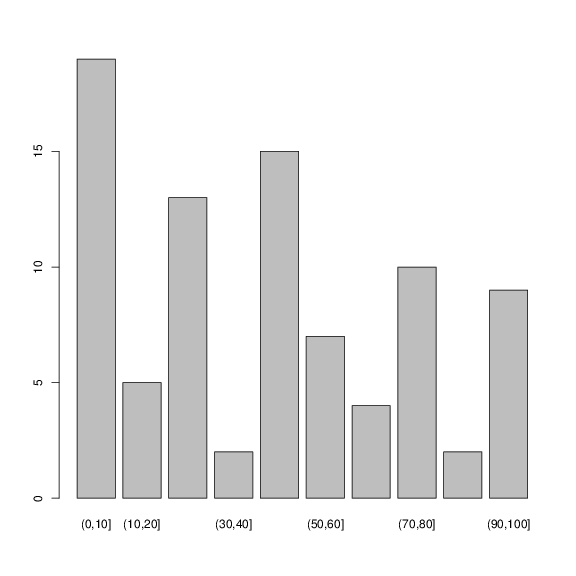
\includegraphics[width=4.5cm]{cancerdist.png}
\end{center}
    \end{column}
    \begin{column}{0.5\textwidth}
\begin{center}
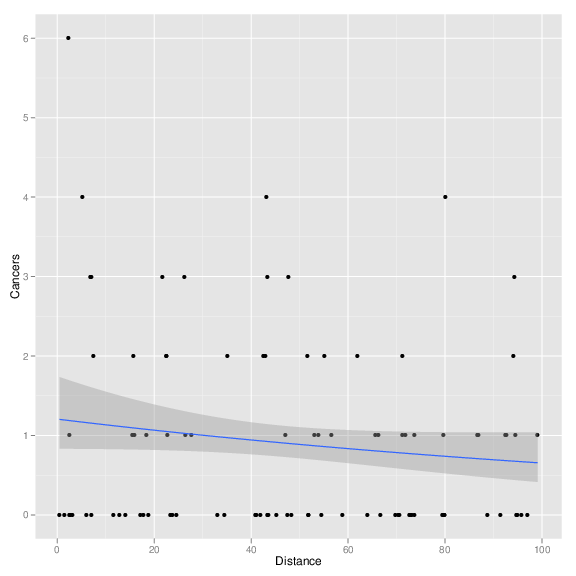
\includegraphics[width=4.5cm]{cancerdist2.png}
\end{center}
    \end{column}
  \end{columns}

\end{frame}

\begin{frame}[fragile]\frametitle{Count Data}
  \begin{itemize}
  \item There seems to be a downward trend in cancer cases with distance. But is the trend significant?\footnotesize
\begin{verbatim}
> m <- glm(Cancers~Distance,family=poisson,data=cancer)
> summary(m)
Call:
glm(formula = Cancers ~ Distance, family = poisson, 
                                     data = cancer)

Deviance Residuals: 
    Min       1Q   Median       3Q      Max  
-1.5504  -1.3491  -1.1553   0.3877   3.1304  
Coefficients:
             Estimate Std. Error z value Pr(>|z|)  
(Intercept)  0.186865   0.188728   0.990   0.3221  
Distance    -0.006138   0.003667  -1.674   0.0941 .
(Dispersion parameter for poisson family taken to be 1)

    Null deviance: 149.48  on 93  degrees of freedom
Residual deviance: 146.64  on 92  degrees of freedom
AIC: 262.41
\end{verbatim}
  \end{itemize}
\end{frame}


\begin{frame}[fragile]\frametitle{Count Data}
  \begin{itemize}
  \item The trend does not look to be significant, but look at the residual deviance:
  \item It is assumed that this is the same as the residual degrees of freedom (because the errors are supposed to be Poisson distributed) 
  \item this indicates that we have overdispersion (extra, unexplained variation in the response). 
  \item we compensate for the overdispersion by refitting the model using quasi-Poisson rather than Poisson errors
  \end{itemize}
\end{frame}

\begin{frame}[fragile]\frametitle{Count Data}
  \begin{itemize}
\item the refitted model\footnotesize
\begin{verbatim}
> m <- glm(Cancers~Distance,family=quasipoisson,data=cancer)
> summary(m)
Call:
glm(formula = Cancers ~ Distance, 
               family = quasipoisson, data = cancer)
Deviance Residuals: 
    Min       1Q   Median       3Q      Max  
-1.5504  -1.3491  -1.1553   0.3877   3.1304  

Coefficients:
             Estimate Std. Error t value Pr(>|t|)
(Intercept)  0.186865   0.235364   0.794    0.429
Distance    -0.006138   0.004573  -1.342    0.183

(Dispersion parameter for quasipoisson family 
                                 taken to be 1.555271)
    Null deviance: 149.48  on 93  degrees of freedom
Residual deviance: 146.64  on 92  degrees of freedom
\end{verbatim}
  \end{itemize}
\end{frame}

\begin{frame}[fragile]\frametitle{Interpreting the Coefficients}
  \begin{itemize}
  \item the estimates remained the same, but the p-vals changed
  \item so there is no compelling evidence to support the existence of a trend in cancer incidence with distance
from the nuclear plant (this is a completely made up example, neither considering varying population nor clinic density)
  \end{itemize}
\end{frame}


\begin{frame}[fragile]\frametitle{Interpreting the Coefficients}
  \begin{itemize}
  \item if you use glms with Poisson errors, the default link function is \texttt{log}
  \item so the parameter estimates and the predictions from the model (the ‘linear predictor’) are in logs, and need to be antilogged
  \item so we have the following following formula for our model
$$\mbox{count}=\exp{(0.186865 - 0.006138 \cdot \mbox{Distance})}$$
  \item antilog the intercept:
\begin{verbatim}
  > exp(coef(m)[1])
(Intercept) 
   1.205464 
\end{verbatim}
\item get 1.2 expected cases at a distance of zero
  \end{itemize}
\end{frame}

\begin{frame}[fragile]\frametitle{Interpreting the Coefficients}
  \begin{itemize}
\item the slope for \texttt{Distance} is a bit easier to interpret than with a logit link
\begin{verbatim}
> exp(coef(m)[2])
 Distance 
0.9938805 
\end{verbatim}
means that for every additional km distance you get 0.006 less cancer cases  (it is nicer to say for every 10 km the expected count of cancer cases decreases by 6\%)
  \end{itemize}
\end{frame}

\begin{frame}[fragile]\frametitle{Interpreting the Coefficients}
  \begin{itemize}
\item again, the \texttt{effects} package is very helpful to give an overview \small
\begin{verbatim}
> allEffects(m,xlevels=list(Distance=seq(0,100,by=10))
+ )
 model: Cancers ~ Distance

 Distance effect
Distance
        0        10        20        30 
1.2054642 1.1336940 1.0661968 1.0027182 
       40        50        60        70
0.9430189 0.8868740 0.8340718 0.7844133
       80        90       100 
0.7377114 0.6937900 0.6524835 
\end{verbatim}
  \end{itemize}
\end{frame}

\begin{frame}[fragile]\frametitle{Interpreting the Coefficients}
  \begin{itemize}
  \item now the effect plot and the (non-significant) fitted line can be drawn
  \end{itemize}
\begin{center}
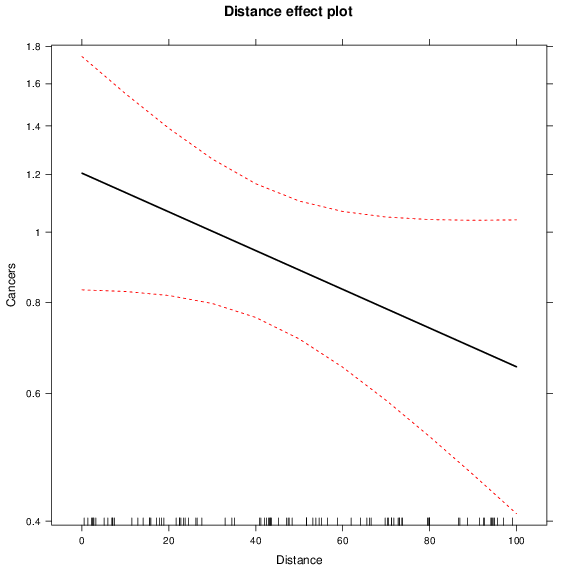
\includegraphics[width=6cm]{cancerdist3.png}
\end{center}
\end{frame}

\begin{frame}[fragile]\frametitle{Interpreting the Coefficients}
\begin{center}
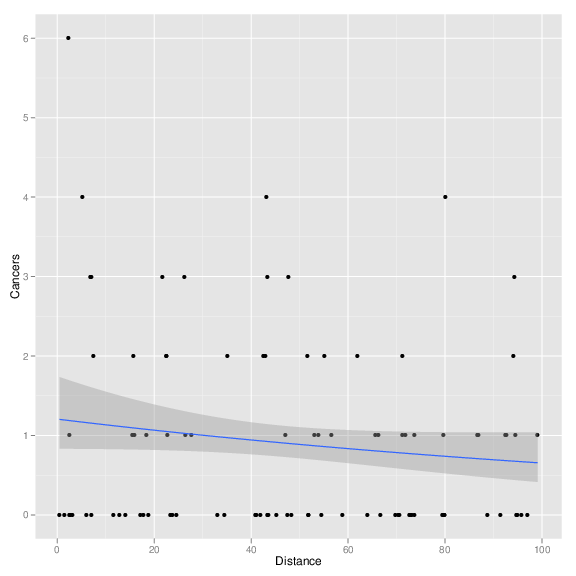
\includegraphics[width=6cm]{cancerdist2.png}
\end{center}
\end{frame}

\begin{frame}[fragile]\frametitle{Anova with Count Data}
\begin{itemize}
\item next example the response variable is a count of infected blood cells per $\mbox{mm}^2$ on microscope slides prepared from randomly selected individuals
\item explanatory variables are smoker (logical, yes or no)
\item and body mass score (three levels, normal, overweight, obese)
\item so we fit the following model (including the interaction term)\tiny
\end{itemize}
\end{frame}


\begin{frame}[fragile]\frametitle{Anova with Count Data}
\footnotesize
\begin{verbatim}
> m <- glm(cells~smoker*weight,family=poisson,data=cells)
> summary(m)
Call:
glm(formula = cells ~ smoker * weight, family = poisson, data = cells)
Deviance Residuals: 
    Min       1Q   Median       3Q      Max  
-2.6511  -1.1742  -0.9148   0.5533   3.6436  
Coefficients:           Estimate Std. Error z value Pr(>|z|)    
(Intercept)             -0.8712     0.1302  -6.692 2.20e-11 ***
smokerTRUE               0.8224     0.1833   4.486 7.27e-06 ***
weightobese              0.4993     0.1671   2.987 0.002817 ** 
weightover               0.2618     0.1866   1.404 0.160465    
smokerTRUE:weightobese   0.8063     0.2296   3.511 0.000446 ***
smokerTRUE:weightover    0.4935     0.2546   1.939 0.052548 .  

(Dispersion parameter for poisson family taken to be 1)
    Null deviance: 1052.95  on 510  degrees of freedom
Residual deviance:  792.85  on 505  degrees of freedom
AIC: 1318.5
\end{verbatim}
\end{frame}




\begin{frame}[fragile]\frametitle{Anova with Count Data}
  \begin{itemize}
  \item again we see overdispersion (residual deviance $>$ degrees of freedom)
  \item we compensate by refitting the model using quasi-Poisson errors
  \end{itemize}
\end{frame}


\begin{frame}[fragile]\frametitle{Anova with Count Data}
\footnotesize
\begin{verbatim}
> m <- glm(cells~smoker*weight,family=quasipoisson,data=cells)
> summary(m)
Call:
glm(formula = cells ~ smoker * weight, family = quasipoisson, 
    data = cells)
Deviance Residuals: 
    Min       1Q   Median       3Q      Max  
-2.6511  -1.1742  -0.9148   0.5533   3.6436  
Coefficients:
                       Estimate Std. Error t value Pr(>|t|)    
(Intercept)             -0.8712     0.1760  -4.950 1.01e-06 ***
smokerTRUE               0.8224     0.2479   3.318 0.000973 ***
weightobese              0.4993     0.2260   2.209 0.027598 *  
weightover               0.2618     0.2522   1.038 0.299723    
smokerTRUE:weightobese   0.8063     0.3105   2.597 0.009675 ** 
smokerTRUE:weightover    0.4935     0.3442   1.434 0.152226    

(Dispersion parameter for quasipoisson family taken to be 1.827927)
\end{verbatim}
\end{frame}

\begin{frame}[fragile]\frametitle{Interpreting the Coefficients}\footnotesize
  \begin{itemize}
\item remember poisson has log as link so
\begin{verbatim}
> exp(coef(m)[1])
(Intercept) 
  0.4184397 
\end{verbatim}
is the expected count of infected blood cells for a normal weighted non-smoker
\item all the other estimates are interpretable as factors (because of the log link!)
\item so a smoker has 
\begin{verbatim}
> exp(coef(m)[2])
smokerTRUE 
  2.276029 
\end{verbatim}
more than twice as many infected cells which is
\begin{verbatim}
> exp(coef(m)[1])*exp(coef(m)[2])
(Intercept) 
   0.952381 
\end{verbatim}
expected infected cells, etc. pp
  \end{itemize}
\end{frame}

\begin{frame}[fragile]\frametitle{Interpreting the Coefficients}
  \begin{itemize}
  \item unfortunately \texttt{effect()} does not work on our model object, so we use \texttt{tapply()} (for simple models a good alternative, as soon as I remove an interaction term, or nested effects this does not work anymore)\footnotesize
\begin{verbatim}
> with(cells,tapply(cells,list(smoker,weight),mean))
         normal     obese      over
FALSE 0.4184397 0.6893939 0.5436893
TRUE  0.9523810 3.5142857 2.0270270
\end{verbatim}
  \end{itemize}
\end{frame}


\begin{frame}[fragile]\frametitle{Interpreting the Coefficients}
  \begin{itemize}
  \item for visualization we use barplot with errorbars indicating the standard error
  \end{itemize}
\begin{center}
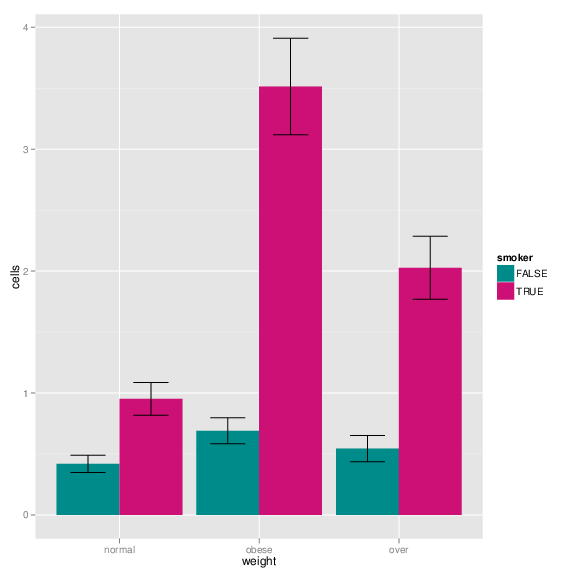
\includegraphics[width=7cm]{obesesmokers.png}
\end{center}
\end{frame}

\begin{frame}[fragile]\frametitle{Ancova with Count Data}
  \begin{itemize}
  \item last example: analysis of covariance
  \item response is a count of the number of plant species on plots 
  \item that have different biomass (a continuous explanatory variable) and
  \item different soil pH (a categorical variable with three levels: high, mid and low)
\begin{verbatim}
> species<-read.table("species.txt",header=T)
> head(species)
    pH   Biomass Species
1 high 0.4692972      30
2 high 1.7308704      39
3 high 2.0897785      44
4 high 3.9257871      35
5 high 4.3667927      25
6 high 5.4819747      29
\end{verbatim}
  \end{itemize}
\end{frame}

\begin{frame}[fragile]\frametitle{Ancova with Count Data}
  \begin{itemize}
  \item this time we begin with a scatter plot\small
\begin{verbatim}
p <- ggplot(species,aes(x=Biomass,y=Species,
+                         shape=pH,colour=pH)) +
     geom_point()
\end{verbatim}
  \end{itemize}
\begin{center}
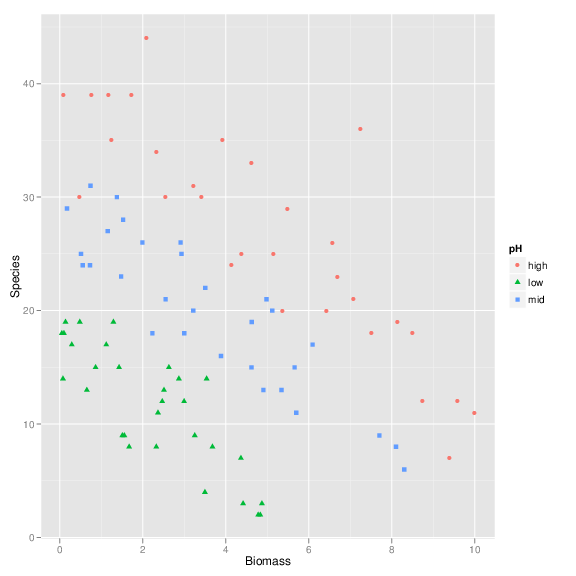
\includegraphics[width=4.5cm]{species.png}
\end{center}
\end{frame}

\begin{frame}[fragile]\frametitle{Ancova with Count Data}
  \begin{itemize}
\item we see: number of species declines with Biomass
\item soil pH has a big effect on Species 
\item Does the slope of the relationship between Species and Biomass depend
on pH?
  \end{itemize}
\end{frame}


\begin{frame}[fragile]\frametitle{Ancova with Count Data}
  \begin{itemize}
  \item define the model and look at the summary\small
\begin{verbatim}
> m <- glm(Species~Biomass*pH,family=poisson,data=species)
> summary(m)
...
Coefficients:
              Estimate Std. Error z value Pr(>|z|)    
(Intercept)    3.76812    0.06153  61.240  < 2e-16 ***
Biomass       -0.10713    0.01249  -8.577  < 2e-16 ***
pHlow         -0.81557    0.10284  -7.931 2.18e-15 ***
pHmid         -0.33146    0.09217  -3.596 0.000323 ***
Biomass:pHlow -0.15503    0.04003  -3.873 0.000108 ***
Biomass:pHmid -0.03189    0.02308  -1.382 0.166954    
...
\end{verbatim}
  \end{itemize}
\end{frame}

\begin{frame}[fragile]\frametitle{Ancova with Count Data}
  \begin{itemize}
  \item test for the need for different slopes by comparing this maximal model (with
six parameters) with a simpler model with different intercepts but the same slope
\begin{verbatim}
> m2 <- glm(Species~Biomass+pH,
+                 family=poisson,data=species)
> anova(m,m2,test="Chi")
Analysis of Deviance Table

Model 1: Species ~ Biomass * pH
Model 2: Species ~ Biomass + pH
  Resid. Df Resid. Dev Df Deviance  Pr(>Chi)    
1        84     83.201                          
2        86     99.242 -2   -16.04 0.0003288 ***
\end{verbatim}
\item AIC: m: 514.4; m2: 526.4 
  \end{itemize}
\end{frame}

\begin{frame}[fragile]\frametitle{Ancova with Count Data}
  \begin{itemize}
  \item slopes are very significantly different $p = 0.00033$ , so it is justified to retain the more complicated model
  \item finally, we have a look on the effects and then draw the fitted lines through the scatterplot using the plot object \texttt{p} from above
  \end{itemize}\small
\begin{verbatim}
> allEffects(m,xlevels=list(Biomass=1:10))
 model: Species ~ Biomass * pH
 Biomass*pH effect
       pH
Biomass     high       low       mid
     1  38.89998 14.737487 27.048707
     2  34.94810 11.338867 23.538030
     3  31.39769  8.724005 20.483007
     4  28.20797  6.712158 17.824498
     5  25.34229  5.164264 15.511039
     6  22.76775  3.973330 13.497847
     ....
\end{verbatim}
\end{frame}

\begin{frame}[fragile]\frametitle{Ancova with Count Data}
  \begin{columns}
    \begin{column}{0.5\textwidth}
\begin{center}
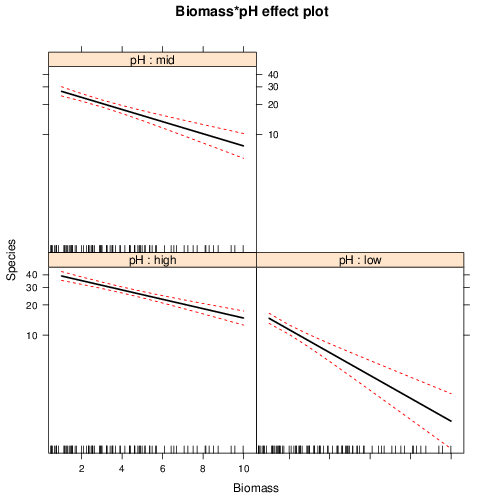
\includegraphics[width=4.5cm]{species2.png}
\end{center}
    \end{column}
    \begin{column}{0.5\textwidth}
\begin{center}
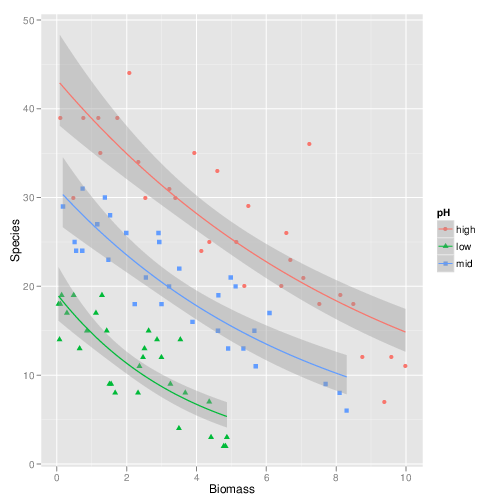
\includegraphics[width=4.5cm]{species3.png}
\end{center}
    \end{column}
  \end{columns}
\end{frame}

\section{Count Data on Proportions}
\begin{frame}[fragile]\frametitle{Proportion Data}
  \begin{itemize}
  \item For comparisons of one binomial proportion with a constant, use \texttt{binom.test()}
  \item For comparison of two samples of proportion data, use \texttt{prop.test()}
  \item The use of GLMs on proportion data is for complex models
  \end{itemize}
\end{frame}

\begin{frame}[fragile]\frametitle{GLMs \& Proportion Data}
  \begin{itemize}
  \item uses also logit as link function and binomial error distribution
  \item if there is overdispersion use quasibinomial to compensate
  \item fitted values are counts
  \item we have seen one example so far: in the challenger example we have already used the responds variable in form of a proportion
  \end{itemize}
\end{frame}

\begin{frame}[fragile]\frametitle{GLMs \& Proportion Data}
  \begin{itemize}
  \item we use an example concerning sex ratios in insects as response and
  \item population density as explanatory variable
  \item so load the data and fit the model
\begin{verbatim}
> numbers <-read.table("sexratio.txt",header=T)
> head(numbers)
  density females males
1       1       1     0
2       4       3     1
3      10       7     3
4      22      18     4
5      55      22    33
6     121      41    80
> m <- glm(cbind(males,females)~density,
+                  family=binomial,data=numbers)
\end{verbatim}
  \end{itemize}
\end{frame}

\begin{frame}[fragile]\frametitle{GLMs \& Proportion Data}\footnotesize
\begin{verbatim}
> summary(m)
Call:
glm(formula = cbind(males, females) ~ density, family = binomial, 
    data = numbers)

Deviance Residuals: 
    Min       1Q   Median       3Q      Max  
-3.4619  -1.2760  -0.9911   0.5742   1.8795  

Coefficients:
             Estimate Std. Error z value Pr(>|z|)    
(Intercept) 0.0807368  0.1550376   0.521    0.603    
density     0.0035101  0.0005116   6.862 6.81e-12 ***

(Dispersion parameter for binomial family taken to be 1)
    Null deviance: 71.159  on 7  degrees of freedom
Residual deviance: 22.091  on 6  degrees of freedom
AIC: 54.618
\end{verbatim}
\end{frame}

\begin{frame}[fragile]\frametitle{GLMs \& Proportion Data}
  \begin{itemize}
  \item the residual deviance is larger than the residual degrees of freedom
  \item because it is something like a growth process we try a log transformation (before using quasibinomial family)\tiny
\begin{verbatim}
> m <- glm(cbind(males,females)~log(density),
+                           family=binomial,data=numbers)
> summary(m)
Call:
glm(formula = cbind(males, females) ~ log(density), 
                   family = binomial, data = numbers)
Deviance Residuals: 
    Min       1Q   Median       3Q      Max  
-1.9697  -0.3411   0.1499   0.4019   1.0372  

Coefficients:
             Estimate Std. Error z value Pr(>|z|)    
(Intercept)  -2.65927    0.48758  -5.454 4.92e-08 ***
log(density)  0.69410    0.09056   7.665 1.80e-14 ***

    Null deviance: 71.1593  on 7  degrees of freedom
Residual deviance:  5.6739  on 6  degrees of freedom
AIC: 38.201
\end{verbatim}
  \end{itemize}
\end{frame}

\begin{frame}[fragile]\frametitle{GLMs \& Proportion Data}
  \begin{itemize}
  \item the transformation caused a welcome decrease in the residual deviance
  \item we conclude that the proportion of animals that are males increases significantly with
increasing density, and 
\item that the logistic model is linearized by logarithmic transformation of the explanatory variable
  \end{itemize}
\end{frame}

\begin{frame}[fragile]\frametitle{GLMs \& Proportion Data}
\begin{verbatim}
ggplot(numbers, aes(x=log(density),y=males/(males+females))) +
  geom_point() +
  geom_smooth(method=glm,family=binomial)
\end{verbatim}
\begin{center}
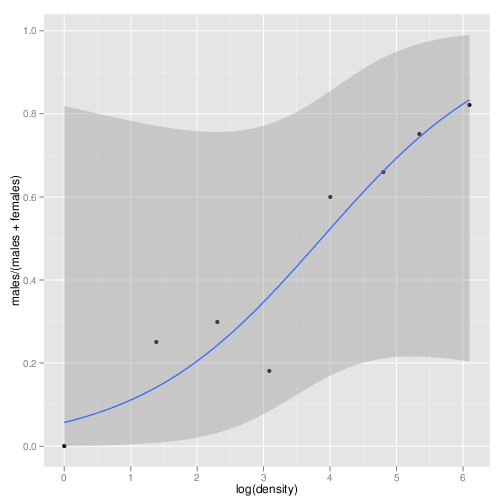
\includegraphics[width=4.5cm]{sexratio.png}
\end{center}
\end{frame}
